\documentclass[
  aps,
  prd,
  reprint,
  superscriptaddress,
  nofootinbib,
  longbibliography
]{revtex4-2}

\usepackage{amsmath,amssymb,bm}
\usepackage{booktabs}
\usepackage{graphicx}
\usepackage{microtype}
\usepackage[hidelinks]{hyperref}

% AUTO-GENERATED by scripts/paper_tex_numbers.py; do not edit.
% Source: docs/research/phase3/numbers.json
% Regenerate: python scripts/paper_tex_numbers.py

% --- Production protocol ---
% numbers.json::production_pulse_A
\newcommand{\PulseAmplitude}{0.10}
% numbers.json::production_pulse_r0
\newcommand{\PulseRadius}{5.0}
% numbers.json::production_pulse_w
\newcommand{\PulseWidth}{1.0}
% numbers.json::production_mexhat_lambda
\newcommand{\MexhatLambda}{0.10}
% numbers.json::production_mexhat_vacuum
\newcommand{\MexhatVacuum}{1.0}
% numbers.json::production_primary_window_lo
\newcommand{\PrimaryWindowLow}{0.10}
% numbers.json::production_primary_window_hi
\newcommand{\PrimaryWindowHigh}{0.50}
% numbers.json::production_primary_order
\newcommand{\PrimaryWindowOrder}{1}
% numbers.json::production_anchor_order
\newcommand{\AnchorWindowOrder}{0}
% numbers.json::production_truth_window_lo
\newcommand{\TruthWindowLow}{0.02}
% numbers.json::production_truth_window_hi
\newcommand{\TruthWindowHigh}{0.20}
% numbers.json::production_truth_order
\newcommand{\TruthWindowOrder}{1}
% numbers.json::production_t_end
\newcommand{\ProductionEndTime}{12.0}
% numbers.json::production_strong_tmin
\newcommand{\StrongTimeLow}{4.0}
% numbers.json::production_strong_tmax
\newcommand{\StrongTimeHigh}{10.0}
% numbers.json::production_strong_fraction
\newcommand{\StrongFraction}{0.30}
% numbers.json::interior_fine_mesh_scale_l0
\newcommand{\FineMeshScaleLZero}{0.028}
% numbers.json::interior_fine_mesh_scale_l2
\newcommand{\FineMeshScaleLTwo}{0.028}
% numbers.json::interior_fine_ladder_rms_linear_l0
\newcommand{\FineLadderRmsLinearLZero}{9.3}
% numbers.json::interior_fine_ladder_rms_mexhat_l0
\newcommand{\FineLadderRmsMexhatLZero}{11.8}
% numbers.json::interior_fine_ladder_rms_linear_l2
\newcommand{\FineLadderRmsLinearLTwo}{19.4}
% numbers.json::interior_fine_ladder_rms_mexhat_l2
\newcommand{\FineLadderRmsMexhatLTwo}{21.4}

% --- R1 interior protocol ---
% numbers.json::interior_domain_radius
\newcommand{\InteriorDomainRadius}{15.0}
% numbers.json::interior_excision_radius
\newcommand{\InteriorExcisionRadius}{0.1}
% numbers.json::interior_outer_mesh_scale
\newcommand{\InteriorOuterMeshScale}{1.2}
% numbers.json::interior_element_degree
\newcommand{\InteriorElementDegree}{1}
% numbers.json::interior_cfl
\newcommand{\InteriorCFL}{0.3}
% numbers.json::interior_extraction_count
\newcommand{\InteriorExtractionCount}{32}
% numbers.json::interior_extraction_r_min
\newcommand{\InteriorExtractionRadiusLow}{0.1}
% numbers.json::interior_extraction_r_max
\newcommand{\InteriorExtractionRadiusHigh}{0.5}
% numbers.json::interior_mesh_scale_coarse
\newcommand{\InteriorMeshScaleCoarse}{0.056}
% numbers.json::interior_mesh_scale_middle
\newcommand{\InteriorMeshScaleMiddle}{0.040}
% numbers.json::interior_mode_l0
\newcommand{\InteriorModeLZero}{0}
% numbers.json::interior_mode_l1
\newcommand{\InteriorModeLOne}{1}
% numbers.json::interior_mode_l2
\newcommand{\InteriorModeLTwo}{2}
% numbers.json::interior_lmax_l0
\newcommand{\InteriorLmaxLZero}{2}
% numbers.json::interior_lmax_l2
\newcommand{\InteriorLmaxLTwo}{4}

% --- R1 exterior protocol ---
% numbers.json::exterior_domain_small
\newcommand{\ExteriorDomainSmall}{20}
% numbers.json::exterior_domain_large
\newcommand{\ExteriorDomainLarge}{40}
% numbers.json::exterior_sponge_small_width
\newcommand{\ExteriorSpongeSmallWidth}{5}
% numbers.json::exterior_sponge_small_onset
\newcommand{\ExteriorSpongeSmallOnset}{15}
% numbers.json::exterior_sponge_large_width
\newcommand{\ExteriorSpongeLargeWidth}{10}
% numbers.json::exterior_sponge_large_onset
\newcommand{\ExteriorSpongeLargeOnset}{30}
% numbers.json::exterior_end_time
\newcommand{\ExteriorEndTime}{70}
% numbers.json::exterior_mesh_scale_coarse
\newcommand{\ExteriorMeshScaleCoarse}{1.4}
% numbers.json::exterior_mesh_scale_middle
\newcommand{\ExteriorMeshScaleMiddle}{1.0}
% numbers.json::exterior_mesh_scale_fine
\newcommand{\ExteriorMeshScaleFine}{0.7}
% numbers.json::exterior_lc_inner_ratio
\newcommand{\ExteriorLcInnerRatio}{3.75}

% --- R1 mechanism ---
% numbers.json::mechanism_rstar_mexhat
\newcommand{\MechanismRstar}{0.625}
% numbers.json::mechanism_rstar_iqr_low
\newcommand{\MechanismRstarIQRLow}{0.414}
% numbers.json::mechanism_rstar_iqr_high
\newcommand{\MechanismRstarIQRHigh}{0.808}
% numbers.json::mechanism_ratio_exponent
\newcommand{\MechanismExponent}{2.79}
% numbers.json::mechanism_ratio_exponent_iqr_low
\newcommand{\MechanismExponentIQRLow}{2.44}
% numbers.json::mechanism_ratio_exponent_iqr_high
\newcommand{\MechanismExponentIQRHigh}{3.29}
% numbers.json::mechanism_ratio_threshold
\newcommand{\MechanismRatioThreshold}{0.01}

% --- R1 interior result ---
% numbers.json::disc_l0_ladder_span_pts
\newcommand{\DiscLadderSpan}{2.1}
% numbers.json::production_budget_low_percent
\newcommand{\ProductionBudgetLow}{10}
% numbers.json::production_budget_high_percent
\newcommand{\ProductionBudgetHigh}{15}

% --- R1 Cowling ---
% numbers.json::cowling_phase0_zeta_max_inside_horizon
\newcommand{\CowlingInsideMaximum}{0.00124}
% numbers.json::cowling_phase0_zeta_at_rmin
\newcommand{\CowlingDeepValue}{0.00016}

% --- R2 sensitivity ---
% numbers.json::sens_lambda_min
\newcommand{\SensitivityLambdaLow}{0.03}
% numbers.json::sens_lambda_boundary
\newcommand{\SensitivityLambdaBoundary}{0.30}
% numbers.json::sens_lambda_max
\newcommand{\SensitivityLambdaHigh}{1.00}
% numbers.json::sens_amplitude_min
\newcommand{\SensitivityAmplitudeLow}{0.01}
% numbers.json::sens_amplitude_max
\newcommand{\SensitivityAmplitudeHigh}{0.10}
% numbers.json::sens_grid_cell_count
\newcommand{\SensitivityGridCount}{12}
% numbers.json::sens_disc_min
\newcommand{\SensitivityDiscLow}{0.712}
% numbers.json::sens_disc_max
\newcommand{\SensitivityDiscHigh}{1.313}
% numbers.json::sens_disc_max_abs_dev
\newcommand{\SensitivityMaxDeviation}{0.313}
% numbers.json::sens_disc_review_threshold
\newcommand{\SensitivityReviewThreshold}{0.15}

% --- Interior discriminator ---
% numbers.json::disc_l0_lc0.028_l2_ratio_frozen
\newcommand{\DiscLZero}{0.923}
% numbers.json::disc_l1_lc0.040_l2_ratio_frozen
\newcommand{\DiscLOne}{0.867}
% numbers.json::disc_l2_lc0.028_l2_ratio_frozen
\newcommand{\DiscLTwo}{0.876}
% numbers.json::disc_oracle_1d_l0_l2_ratio
\newcommand{\DiscOracle}{1.006}
% numbers.json::disc_l0_lc0.028_ratio_median_frozen
\newcommand{\DiscMedianLZero}{0.851}
% numbers.json::disc_l0_lc0.028_ratio_median_frozen
\newcommand{\DiscIQRLowLZero}{0.574}
% numbers.json::disc_l0_lc0.028_ratio_median_frozen
\newcommand{\DiscIQRHighLZero}{1.175}
% numbers.json::disc_l1_lc0.040_ratio_median_frozen
\newcommand{\DiscMedianLOne}{0.640}
% numbers.json::disc_l1_lc0.040_ratio_median_frozen
\newcommand{\DiscIQRLowLOne}{0.329}
% numbers.json::disc_l1_lc0.040_ratio_median_frozen
\newcommand{\DiscIQRHighLOne}{0.884}
% numbers.json::disc_l2_lc0.028_ratio_median_frozen
\newcommand{\DiscMedianLTwo}{0.813}
% numbers.json::disc_l2_lc0.028_ratio_median_frozen
\newcommand{\DiscIQRLowLTwo}{0.488}
% numbers.json::disc_l2_lc0.028_ratio_median_frozen
\newcommand{\DiscIQRHighLTwo}{0.975}
% numbers.json::o1_truth_floor_linear_l1
\newcommand{\TruthFloorLOne}{10.1}
% numbers.json::o1_truth_floor_linear_l2
\newcommand{\TruthFloorLTwo}{6.6}
% numbers.json::linear_l0_lc0.028_dev_primary_median
\newcommand{\FrozenDevLinearFine}{13.1}
% numbers.json::mexhat_l0_lc0.028_dev_primary_median
\newcommand{\FrozenDevMexhatFine}{8.6}
% numbers.json::mass_lumping_ab_dev_median
\newcommand{\LumpingDevMedian}{27.7}
% numbers.json::mass_lumping_ab_dev_max
\newcommand{\LumpingDevMax}{38.6}

% --- Window calibration ---
% numbers.json::o1_c_linear_l0_sampled_k32_median
\newcommand{\OOneCLinearMedian}{1.020}
% numbers.json::o1_c_linear_l0_sampled_k32_median
\newcommand{\OOneCLinearIQRLow}{0.982}
% numbers.json::o1_c_linear_l0_sampled_k32_median
\newcommand{\OOneCLinearIQRHigh}{1.042}
% numbers.json::o1_c_mexhat_l0_sampled_k32_median
\newcommand{\OOneCMexhatMedian}{1.014}
% numbers.json::o1_c_mexhat_l0_sampled_k32_median
\newcommand{\OOneCMexhatIQRLow}{0.993}
% numbers.json::o1_c_mexhat_l0_sampled_k32_median
\newcommand{\OOneCMexhatIQRHigh}{1.069}
% numbers.json::o1_linear_l0_lc0.028_dev_before_common_support
\newcommand{\OOneLinearFineBefore}{10.31}
% numbers.json::o1_linear_l0_lc0.028_dev_residual
\newcommand{\OOneLinearFineResidual}{7.11}
% numbers.json::o1_linear_l0_lc0.028_dev_fraction_explained
\newcommand{\OOneLinearFineFraction}{31.0}
% numbers.json::o1_mexhat_l0_lc0.028_dev_before_common_support
\newcommand{\OOneMexhatFineBefore}{4.83}
% numbers.json::o1_mexhat_l0_lc0.028_dev_residual
\newcommand{\OOneMexhatFineResidual}{3.89}
% numbers.json::o1_mexhat_l0_lc0.028_dev_fraction_explained
\newcommand{\OOneMexhatFineFraction}{19.3}
% numbers.json::o1_deficit_fraction_explained
\newcommand{\OOneDeficitExplained}{31.0}
% numbers.json::o1_remaining_l2_deficit
\newcommand{\OOneDeficitResidual}{4.16}

% --- Off-channel diagnostics ---
% numbers.json::linear_l2_lc0.028_junk_offchannel_l0
\newcommand{\OffLTwoToZeroLinear}{1.95}
% numbers.json::mexhat_l2_lc0.028_junk_offchannel_l0
\newcommand{\OffLTwoToZeroMexhat}{1.89}
% numbers.json::linear_l2_lc0.028_junk_offchannel_l4
\newcommand{\OffLTwoToFourLinear}{3.38}
% numbers.json::mexhat_l2_lc0.028_junk_offchannel_l4
\newcommand{\OffLTwoToFourMexhat}{3.40}
% numbers.json::linear_l1_lc0.040_junk_offchannel_l0
\newcommand{\OffLOneToZeroLinear}{1.61}
% numbers.json::mexhat_l1_lc0.040_junk_offchannel_l0
\newcommand{\OffLOneToZeroMexhat}{3.50}

% --- Exterior protocol ---
% numbers.json::exterior_l
\newcommand{\ExteriorMultipoleL}{2}
% numbers.json::exterior_m
\newcommand{\ExteriorMultipoleM}{0}
% numbers.json::exterior_r_ext
\newcommand{\ExteriorRadius}{6.0}
% numbers.json::exterior_pulse_A
\newcommand{\ExteriorPulseAmplitude}{0.001}
% numbers.json::exterior_pulse_r0
\newcommand{\ExteriorPulseRadius}{8.0}
% numbers.json::exterior_pulse_w
\newcommand{\ExteriorPulseWidth}{2.0}
% numbers.json::exterior_designed_window_length
\newcommand{\ExteriorWindowLength}{26.0}
% numbers.json::exterior_designed_window_t_search
\newcommand{\ExteriorSearchTime}{12.0}
% numbers.json::exterior_designed_window_mode_count
\newcommand{\ExteriorModeCount}{4}
% numbers.json::exterior_tail_tmin
\newcommand{\ExteriorTailTime}{40.0}
% numbers.json::exterior_tail_floor_tmin
\newcommand{\ExteriorFloorTime}{55.0}
% numbers.json::exterior_late_window_length
\newcommand{\ExteriorLateWindowLength}{16.0}
% numbers.json::exterior_late_window_min_offset
\newcommand{\ExteriorLateMinOffset}{10.0}

% --- Exterior results ---
% numbers.json::qnm_leaver_l2_re
\newcommand{\LeaverRe}{0.48364}
% numbers.json::qnm_leaver_l2_minus_im
\newcommand{\LeaverMinusIm}{0.09676}
% numbers.json::qnm_R20_lc0.7_re
\newcommand{\RTwentyFineRe}{0.47455}
% numbers.json::qnm_R20_lc0.7_re_error_signed
\newcommand{\RTwentyFineReError}{-1.88}
% numbers.json::qnm_R20_fine_re_order
\newcommand{\RTwentyFineOrder}{1.77}
% numbers.json::qnm_R40_late_pooled_re
\newcommand{\RFortyLateRe}{0.48772}
% numbers.json::qnm_R40_late_pooled_re
\newcommand{\RFortyLateReUnc}{0.01244}
% numbers.json::qnm_R40_late_pooled_re_error_signed
\newcommand{\RFortyLateReError}{+0.84}
% numbers.json::qnm_R40_late_pooled_minus_im
\newcommand{\RFortyLateMinusIm}{0.10161}
% numbers.json::qnm_R40_late_pooled_minus_im
\newcommand{\RFortyLateMinusImUnc}{0.00545}
% numbers.json::qnm_R40_late_pooled_minus_im_error_signed
\newcommand{\RFortyLateMinusImError}{+5.01}
% numbers.json::qnm_R40_lc1match_early_overtone_bias
\newcommand{\EarlyBiasLcOne}{14.1}
% numbers.json::qnm_R40_lc0.7match_early_overtone_bias
\newcommand{\EarlyBiasLcPointSeven}{15.8}
% numbers.json::domain_R40_lc1match_delta_re
\newcommand{\DomainDeltaRe}{-0.00221}
% numbers.json::domain_R40_lc1match_delta_re
\newcommand{\DomainDeltaReUnc}{0.00582}
% numbers.json::domain_R40_lc1match_tail_floor_reduction
\newcommand{\DomainFloorReductionLcOne}{47.1}
% numbers.json::domain_R40_lc0.7match_tail_floor_reduction
\newcommand{\DomainFloorReductionLcPointSeven}{27.7}
% numbers.json::domain_R40_lc1match_R20_peak_over_floor
\newcommand{\DomainPeakFloorRTwenty}{4.1}
% numbers.json::domain_R40_lc1match_R40_peak_over_floor
\newcommand{\DomainPeakFloorRForty}{195.5}

% --- Cavity doublet ---
% numbers.json::cavity_lc1_w1
\newcommand{\CavityLcOneWOne}{0.3535}
% numbers.json::cavity_lc1_w1
\newcommand{\CavityLcOneWOneUnc}{0.0010}
% numbers.json::cavity_lc1_w2
\newcommand{\CavityLcOneWTwo}{0.5630}
% numbers.json::cavity_lc1_w2
\newcommand{\CavityLcOneWTwoUnc}{0.0040}


\newcommand{\dd}{\mathrm{d}}
\newcommand{\order}{\mathcal{O}}
\newcommand{\ahat}[1]{a_{\mathrm{hat},#1}}
\newcommand{\alin}[1]{a_{\mathrm{lin},#1}}

\begin{document}

\title{Logarithmic scalar-field profiles near the Schwarzschild singularity}

\author{Marco Garc\'ia}

\date{July 12, 2026}

\begin{abstract}
We measure the near-singularity logarithmic profile of test scalar fields
inside a Schwarzschild black hole in three spatial dimensions.  The metric is
held fixed, matching the test-field scope of the rigorous
Fournodavlos--Sbierski asymptotics, while the scalar retains a nonlinear
symmetry-breaking potential.  Identical initial data are evolved with a
finite-element excision scheme and compared mode by mode with a free scalar.
% numbers.json::disc_l0_lc0.028_l2_ratio_frozen
% numbers.json::disc_l1_lc0.040_l2_ratio_frozen
% numbers.json::disc_l2_lc0.028_l2_ratio_frozen
% numbers.json::disc_oracle_1d_l0_l2_ratio
The primary Mexican-hat-to-linear $L^2$ ratios are
$\DiscLZero$, $\DiscLOne$, and $\DiscLTwo$ for the finest available
$l=0,1,2$ runs, respectively, compared with $\DiscOracle$ in the spherical
oracle.  Thus the vacuum structure changes the logarithmic coefficient only
within the quantified numerical error budget rather than changing its
near-singularity scaling.
% numbers.json::o1_truth_floor_linear_l1
% numbers.json::o1_truth_floor_linear_l2
The $l>0$ values remain frozen and uncorrected because their truth-window
floors, $\TruthFloorLOne\%$ and $\TruthFloorLTwo\%$, exceed the correction
being tested.
% numbers.json::o1_deficit_fraction_explained
% numbers.json::o1_remaining_l2_deficit
A profile-dependent window calibration explains $\OOneDeficitExplained\%$
of the monopole $L^2$ deficit on common support and leaves
$\OOneDeficitResidual$ percentage points as a three-dimensional
mesh/extraction systematic; it is diagnostic and does not replace the frozen
ratios.
% numbers.json::qnm_R40_late_pooled_re
% numbers.json::qnm_R40_late_pooled_minus_im
Exterior validation gives
$M\omega=\RFortyLateRe\pm\RFortyLateReUnc
-i(\RFortyLateMinusIm\pm\RFortyLateMinusImUnc)$ from late, large-domain
windows, with scatter dominated by the fitting protocol.  The calculation
therefore supplies a controlled numerical test of kinetic domination in the
black-hole interior, explicitly within the Cowling limit.
\end{abstract}

\maketitle

\section{Introduction}
\label{sec:intro}

For a massless scalar on a fixed Schwarzschild spacetime,
Fournodavlos and Sbierski proved that smooth solutions approaching the
spacelike singularity admit the expansion
\begin{equation}
  \phi(t,r,\Omega)
  = A(t,\Omega)\ln r+B(t,\Omega)+\order(r\lvert\ln r\rvert),
  \label{eq:fs-expansion}
\end{equation}
and that logarithmic blow-up is generic in precise energy topologies
\cite{FournodavlosSbierski2020}.  The coefficient $A$ is a function on the
singular hypersurface rather than a single global amplitude.  Its spherical
harmonic components are the observables $a_l(t)$ studied below.

The theorem is linear, but the approach to a spacelike singularity is often
associated with velocity or kinetic domination.  In self-gravitating
Einstein--scalar systems, monotone, quiescent singular behavior is stable in
broad near-FLRW and subcritical Kasner regimes
\cite{RodnianskiSpeck2018,FournodavlosRodnianskiSpeck2023}.  This motivates a
test-field question with a direct numerical answer: does a nonlinear vacuum
potential retain an observable imprint in $A(t,\Omega)$, or is that structure
washed out as the kinetic terms dominate?

Previous numerical studies provide complementary pieces but not this
measurement.  Thuestad, Khanna, and Price evolved scalar fields through the
interiors of Schwarzschild and Kerr black holes and found interior
$l$-dependent oscillations, without extracting the $r\to0$ logarithmic
coefficient \cite{ThuestadKhannaPrice2017}.  Symmetry-breaking scalars have
also been evolved in the exterior: accretion can delay symmetry breaking near
the horizon \cite{TraykovaBradenPeiris2018} or form symmetry-restored shells
and trigger vacuum decay \cite{MarsdenEtAl2025}.  Black-hole-seeded vacuum
decay itself has a substantial literature, with both catalytic scenarios and
strong counterarguments \cite{BurdaGregoryMoss2015PRL,Strumia2023}.  These
works motivate the physics while leaving the near-singularity profile open.

We present, to our knowledge, the first numerical measurement of
$A(t,\Omega)$ approaching the Schwarzschild singularity and the first
identical-data comparison of its free and symmetry-breaking evolutions.  The
measurement is performed mode by mode in $3+1$ dimensions.  The methodology
is deliberately not claimed as the first scalar evolution with excision:
three-dimensional finite-difference excision predates this work
\cite{CalabreseEtAl2003}, and finite elements have been used for black-hole
perturbations \cite{SopuertaLaguna2006}.  The methodological contribution is
the combination of a DOLFINx finite-element evolution, calibrated multi-radius
interior extraction, paired potential comparison, and an exterior validation
that separates finite-domain and overtone systematics.

Section~\ref{sec:setup} defines the physical problem and its scope.
Section~\ref{sec:numerics} describes the evolution and observables.
Sections~\ref{sec:interior} and \ref{sec:exterior} give the interior and
exterior results, followed by limitations and interpretation in
Sec.~\ref{sec:discussion}.

\section{Physical setup and scope}
\label{sec:setup}

We evolve a real scalar on a Schwarzschild background in ingoing
Kerr--Schild coordinates.  With signature $(-,+,+,+)$,
\begin{equation}
  g_{\mu\nu}=\eta_{\mu\nu}+2H k_\mu k_\nu,
  \qquad H=\frac{M}{r},
  \qquad k_\mu=(1,x_i/r),
  \label{eq:ks-metric}
\end{equation}
which is regular at the event horizon.  Geometrized units $G=c=M=1$ are
used unless $M$ is shown explicitly.

The scalar action and equation of motion are
\begin{align}
  S_\phi
  &= -\int \dd^4x\,\sqrt{-g}
     \left[\frac12 g^{\mu\nu}\partial_\mu\phi\partial_\nu\phi
     +V(\phi)\right], \\
  \Box_g\phi-V'(\phi)&=0.
  \label{eq:kg}
\end{align}
Two models are compared.  The linear member has $V_{\rm lin}=0$.  The
symmetry-breaking member has
\begin{equation}
  V_{\rm hat}(\phi)=\frac{\lambda}{4}(\phi^2-v^2)^2 .
  \label{eq:mexhat}
\end{equation}
% numbers.json::production_mexhat_lambda
% numbers.json::production_mexhat_vacuum
We use $\lambda=\MexhatLambda$ and $v=\MexhatVacuum$, and initialize the
nonlinear field in the vacuum approached at the outer boundary.  The two
members of every comparison receive the same perturbation.

% numbers.json::production_pulse_A
% numbers.json::production_pulse_r0
% numbers.json::production_pulse_w
The production perturbation is an ingoing curved Gaussian with amplitude
$\PulseAmplitude$, center $r_0=\PulseRadius M$, and width
$w=\PulseWidth M$, multiplied by a real $Y_{l0}$.  We evolve $l=0,1,2$.
The angular decomposition is performed numerically in three dimensions; no
spherical symmetry is imposed on the evolution.

The metric is not evolved.  This Cowling or test-field limit is a physical
restriction of the study, not an omitted convergence check.  It is also the
precise background setting of Eq.~\eqref{eq:fs-expansion}.  Our result tests
the effect of $V(\phi)$ on the scalar asymptotics; it does not address
backreaction, mass inflation, or singularity resolution.

\section{Numerical method and observables}
\label{sec:numerics}

\subsection{First-order finite-element evolution}

Writing the metric in $3+1$ form with lapse $\alpha$, shift $\beta^i$,
spatial metric $\gamma_{ij}$, and extrinsic-curvature trace $K$, we define
\begin{equation}
  \Pi=\alpha^{-1}(\partial_t\phi-\beta^i\partial_i\phi).
\end{equation}
The evolved system is
\begin{align}
  \partial_t\phi
    &=\alpha\Pi+\beta^i\partial_i\phi, \\
  \partial_t\Pi
    &=\alpha D_iD^i\phi+D^i\alpha D_i\phi
      +\beta^i\partial_i\Pi+\alpha K\Pi-\alpha V'(\phi).
  \label{eq:first-order}
\end{align}
We discretize both variables with continuous piecewise-linear elements on a
graded tetrahedral Gmsh mesh \cite{GeuzaineRemacle2009} and assemble the weak
form in DOLFINx \cite{BarattaEtAl2023}.  Time integration uses SSP-RK3.
The black-hole interior is excised inside the horizon, where no incoming
characteristic requires inner boundary data.  At the outer boundary we use a
characteristic radiative condition; exterior spectroscopy additionally uses
a smooth damping layer.

We record the Killing-energy change together with the inner and outer fluxes
as an implementation diagnostic.  Its production residual is dominated by
surface quadrature on the faceted excision boundary, so it is not promoted as
a field-accuracy metric; convergence of the evolved field and the paired
profile observables is assessed separately.

The linear operator is preassembled.  Only the cubic part of
$V'_{\rm hat}=\lambda\phi(\phi^2-v^2)$ is assembled at each stage.
The consistent mass matrix is retained in production.
% numbers.json::mass_lumping_ab_dev_median
% numbers.json::mass_lumping_ab_dev_max
A direct A/B test found that row-sum mass lumping displaced the interior
observable by $\LumpingDevMedian\%$ in the median and $\LumpingDevMax\%$ at
maximum.  It was therefore rejected despite its computational speed.

\subsection{Near-singularity estimator}

Following the full hierarchy associated with Eq.~\eqref{eq:fs-expansion},
the primary radial model for each multipole is
\begin{equation}
  \phi_l(t,r)
  \simeq a_l(t)\ln r+b_l(t)
  +c_l(t)r\ln r+d_l(t)r .
  \label{eq:o1-fit}
\end{equation}
% numbers.json::production_primary_window_lo
% numbers.json::production_primary_window_hi
% numbers.json::production_primary_order
The fit is performed over
$r/M\in[\PrimaryWindowLow,\PrimaryWindowHigh]$ with truncation order
$\PrimaryWindowOrder$.  A lower-order fit over the same radii supplies only
the phase anchor.  The primary order is a bias--variance compromise: higher
orders reduce the one-dimensional truncation bias but amplify correlated
three-dimensional mesh errors.

% numbers.json::production_strong_tmin
% numbers.json::production_strong_tmax
% numbers.json::production_strong_fraction
Statistics use the anchored strong phase
$t/M\in[\StrongTimeLow,\StrongTimeHigh]$ and require the anchor magnitude to
exceed $\StrongFraction$ of its maximum in that interval.  This upper time
cut removes late finite-domain contamination.  For one-dimensional truth we
use the same asymptotic order on a deeper interval,
% numbers.json::production_truth_window_lo
% numbers.json::production_truth_window_hi
% numbers.json::production_truth_order
$r/M\in[\TruthWindowLow,\TruthWindowHigh]$ at order
$\TruthWindowOrder$.

\subsection{Paired discriminator and calibration}

The primary identical-data discriminator for each $l$ is
\begin{equation}
  \mathcal{D}_l
  =\frac{\lVert \ahat{l}\rVert_{2,\mathcal{S}}}
  {\lVert \alin{l}\rVert_{2,\mathcal{S}}},
  \label{eq:discriminator}
\end{equation}
where $\mathcal{S}$ is the common strong support.  The median and interquartile
range of $\ahat{l}/\alin{l}$ are secondary summaries.  Pointwise ratios near a
zero crossing are ill-conditioned.  Ratios of separate maxima are excluded
because the maxima occur at different times and inherit a differential
window bias.

For $l=0$, a diagnostic calibration is obtained by applying the production
fit and the deeper truth fit to the same dense oracle snapshot,
\begin{equation}
  c_X(t)=\frac{a_{X,\mathrm{prod}}(t)}{a_{X,\mathrm{truth}}(t)}.
  \label{eq:calibration}
\end{equation}
The ratio is defined only in the oracle strong phase and is never filled
across its zero-crossing gap or beyond its support.  Corrections are applied
to both members of a pair before recomputing a diagnostic discriminator.
They do not replace the frozen production values.

\section{Interior results}
\label{sec:interior}

\subsection{Logarithmic profiles}

Figure~\ref{fig:profiles} compares the three-dimensional monopole profiles
with the dense spherical oracle and Eq.~\eqref{eq:o1-fit}.  The curves are
approximately affine in $\ln r$, and the same basis describes both
potentials across representative parts of the common strong phase.

\begin{figure*}
  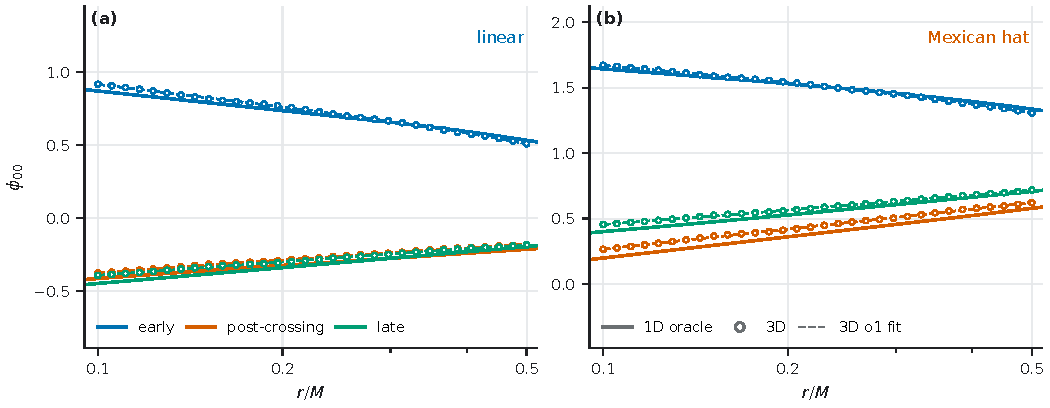
\includegraphics[width=\textwidth]{figures/interior_profiles.pdf}
  \caption{Near-singularity monopole profiles for identical initial data in
  the linear and Mexican-hat models.  Solid curves show the dense spherical
  oracle, open circles the versioned low-resolution $3+1$D profile bank, and dashed
  curves the primary order-one fits.  Colors select reproducible
  representatives of the common strong phase.  This is a qualitative
  low-resolution profile comparison; quantitative deviations and the
  $L^2$ discriminator are reported separately.}
  \label{fig:profiles}
\end{figure*}

% numbers.json::linear_l0_lc0.028_dev_primary_median
% numbers.json::mexhat_l0_lc0.028_dev_primary_median
At the finest production rung, the median three-dimensional-to-oracle
deviation is $\FrozenDevLinearFine\%$ for the linear field and
$\FrozenDevMexhatFine\%$ for the Mexican-hat field.  These comparisons
include temporal interpolation and extraction floors; they are not pure mesh
uncertainties.

\subsection{Identical-data discriminator}

The mode-by-mode result is summarized in Table~\ref{tab:disc} and
Fig.~\ref{fig:disc}.  In every mode the nonlinear coefficient remains of the
same order as its linear partner.  This is the operational signature of
vacuum-structure erasure: the potential changes amplitudes within the
numerical budget but does not introduce a distinct near-singularity scaling.

\begin{table}
  \caption{Frozen $L^2$ discriminator at the finest available rung.  The
  $l>0$ values are not calibration-corrected; their truth-window floors are
  stated in the text.}
  \label{tab:disc}
  \begin{ruledtabular}
  \begin{tabular}{c@{\quad}cc}
    $l$ & $\mathcal{D}_l$ & median [IQR] \\
    \hline
    % numbers.json::disc_l0_lc0.028_l2_ratio_frozen
    % numbers.json::disc_l0_lc0.028_ratio_median_frozen
    $0$ & $\DiscLZero$ & $\DiscMedianLZero$
      [$\DiscIQRLowLZero,\DiscIQRHighLZero$] \\
    % numbers.json::disc_l1_lc0.040_l2_ratio_frozen
    % numbers.json::disc_l1_lc0.040_ratio_median_frozen
    $1$ & $\DiscLOne$ & $\DiscMedianLOne$
      [$\DiscIQRLowLOne,\DiscIQRHighLOne$] \\
    % numbers.json::disc_l2_lc0.028_l2_ratio_frozen
    % numbers.json::disc_l2_lc0.028_ratio_median_frozen
    $2$ & $\DiscLTwo$ & $\DiscMedianLTwo$
      [$\DiscIQRLowLTwo,\DiscIQRHighLTwo$] \\
  \end{tabular}
  \end{ruledtabular}
\end{table}

\begin{figure*}
  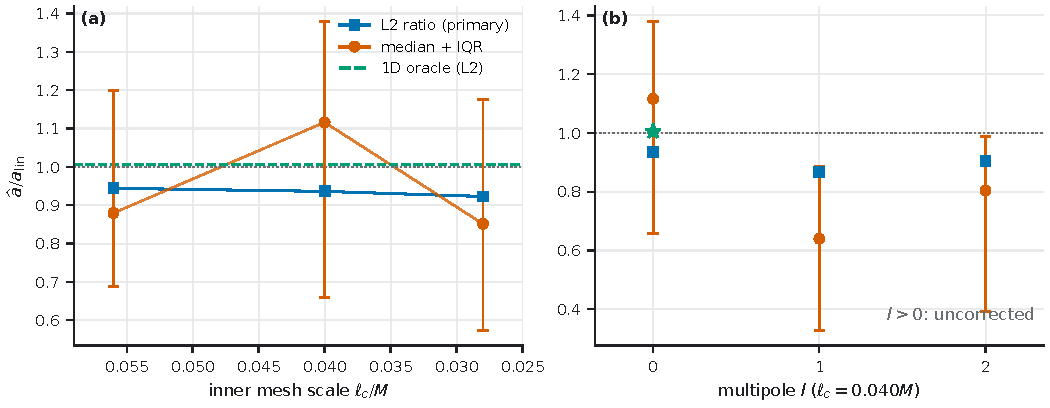
\includegraphics[width=\textwidth]{figures/interior_discriminator.pdf}
  \caption{Identical-data Mexican-hat-to-linear discriminator.  Squares show
  the frozen $L^2$ ratio, the primary statistic; circles and bars show the
  secondary median and IQR.  The dashed line is the spherical-oracle $L^2$
  ratio.  The $l>0$ values are frozen and uncorrected because their
  truth-window floors exceed the correction being tested.  Peak ratios and
  corrected common-support $L^2$ diagnostics are deliberately omitted.}
  \label{fig:disc}
\end{figure*}

% numbers.json::o1_truth_floor_linear_l1
% numbers.json::o1_truth_floor_linear_l2
For $l=1$ and $l=2$, the truth-window floors are $\TruthFloorLOne\%$ and
$\TruthFloorLTwo\%$, respectively.  They are comparable to or larger than
the effect one would attempt to correct, so promoting either an intrinsic or
transferred $l>0$ correction would add unjustified precision.
% numbers.json::interior_fine_ladder_rms_linear_l0
% numbers.json::interior_fine_ladder_rms_mexhat_l0
The fine-rung RMS differences for the individual monopole series are
$\FineLadderRmsLinearLZero\%$ and $\FineLadderRmsMexhatLZero\%$ for the
linear and nonlinear runs.  Their paired discriminator is visibly more
stable than either absolute comparison because the members share the mesh,
estimator, and initial data.

\subsection{Profile-dependent window systematic}

% numbers.json::o1_c_linear_l0_sampled_k32_median
% numbers.json::o1_c_mexhat_l0_sampled_k32_median
On their oracle strong phases, the sampled calibration factors have medians
$\OOneCLinearMedian$ [$\OOneCLinearIQRLow,\OOneCLinearIQRHigh$] and
$\OOneCMexhatMedian$ [$\OOneCMexhatIQRLow,\OOneCMexhatIQRHigh$] for the
linear and Mexican-hat profiles.  Figure~\ref{fig:o1} displays their time
dependence and the strict-support deviation budget.

\begin{figure*}
  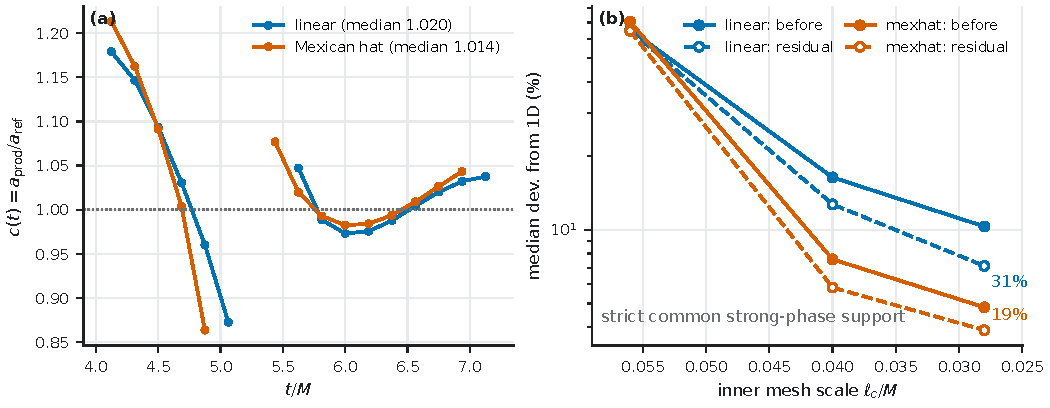
\includegraphics[width=\textwidth]{figures/o1_calibration.pdf}
  \caption{Window calibration of the monopole estimator.  Left: $c(t)$ for
  the linear and Mexican-hat oracles, defined only on strong-phase support
  and left unfilled elsewhere.  Right: median 3D--1D deviation before and
  after the diagnostic calibration on strict common support.  Residual
  curves do not replace the frozen production deviations; the coarsest rung
  is shown diagnostically and is not used for a convergence claim.}
  \label{fig:o1}
\end{figure*}

% numbers.json::o1_linear_l0_lc0.028_dev_before_common_support
% numbers.json::o1_linear_l0_lc0.028_dev_residual
% numbers.json::o1_linear_l0_lc0.028_dev_fraction_explained
For the fine linear run the common-support median deviation changes from
$\OOneLinearFineBefore\%$ to $\OOneLinearFineResidual\%$, accounting for
$\OOneLinearFineFraction\%$ of that median deviation.
% numbers.json::o1_mexhat_l0_lc0.028_dev_before_common_support
% numbers.json::o1_mexhat_l0_lc0.028_dev_residual
% numbers.json::o1_mexhat_l0_lc0.028_dev_fraction_explained
The corresponding Mexican-hat values are $\OOneMexhatFineBefore\%$,
$\OOneMexhatFineResidual\%$, and $\OOneMexhatFineFraction\%$.
These are systematic diagnostics on reduced support, not substitutes for the
production values quoted above.

\subsection{Off-channel response}

Nonlinear mode coupling is constrained by comparing each off-channel signal
with its linear control over the same capped strong phase.
% numbers.json::linear_l2_lc0.028_junk_offchannel_l0
% numbers.json::mexhat_l2_lc0.028_junk_offchannel_l0
% numbers.json::linear_l2_lc0.028_junk_offchannel_l4
% numbers.json::mexhat_l2_lc0.028_junk_offchannel_l4
For the fine $l=2$ pair, the $l=0$ off-channel fractions are
$\OffLTwoToZeroLinear\%$ (linear) and $\OffLTwoToZeroMexhat\%$ (nonlinear),
while the $l=4$ fractions are $\OffLTwoToFourLinear\%$ and
$\OffLTwoToFourMexhat\%$.  The pairs are indistinguishable at this level.
% numbers.json::linear_l1_lc0.040_junk_offchannel_l0
% numbers.json::mexhat_l1_lc0.040_junk_offchannel_l0
The $l=1\to0$ pair changes from $\OffLOneToZeroLinear\%$ to
$\OffLOneToZeroMexhat\%$ and is the only weak excess.  Only an excess over
the paired linear junk constrains coupling; no isolated fraction is treated
as a detection.

\section{Exterior validation}
\label{sec:exterior}

We validate the same three-dimensional evolution and extraction stack using
the fundamental scalar $l=2$ Schwarzschild quasinormal mode.  The reference
frequency is obtained independently by the Leaver continued-fraction method
\cite{Leaver1985}.
% numbers.json::qnm_leaver_l2_re
% numbers.json::qnm_leaver_l2_minus_im
Its value is
$M\omega_{\rm L}=\LeaverRe-i\LeaverMinusIm$.

% numbers.json::exterior_l
% numbers.json::exterior_m
% numbers.json::exterior_r_ext
We excite $(l,m)=(\ExteriorMultipoleL,\ExteriorMultipoleM)$ and extract at
$r=\ExteriorRadius M$.
% numbers.json::exterior_pulse_A
% numbers.json::exterior_pulse_r0
% numbers.json::exterior_pulse_w
The exterior pulse has amplitude $\ExteriorPulseAmplitude$, center
$\ExteriorPulseRadius M$, and width $\ExteriorPulseWidth M$.
% numbers.json::exterior_designed_window_length
% numbers.json::exterior_designed_window_t_search
% numbers.json::exterior_designed_window_mode_count
The designed fit uses peak-anchored windows of length
$\ExteriorWindowLength M$, begins its peak search at
$\ExteriorSearchTime M$, and permits $\ExteriorModeCount$ Prony modes.

\subsection{Real frequency and damping}

Figure~\ref{fig:qnm} separates two effects that a single window average would
mix: mesh behavior of the real frequency and first-overtone bias of the
damping rate.

\begin{figure*}
  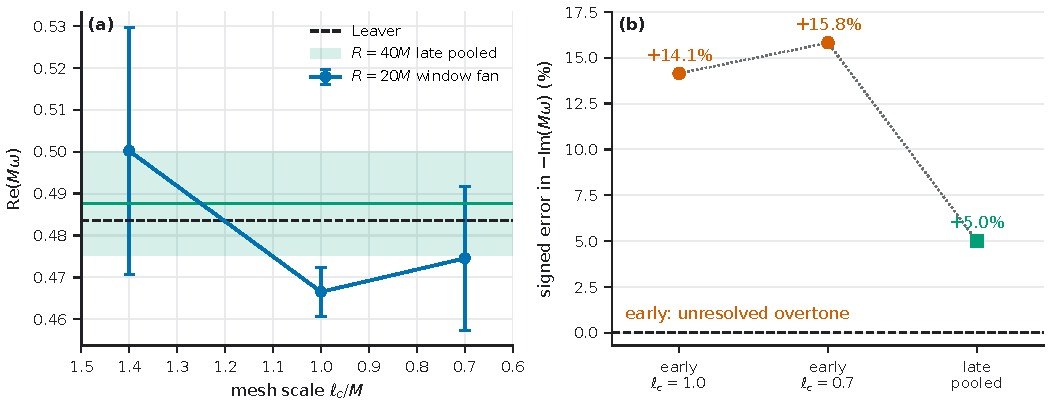
\includegraphics[width=\textwidth]{figures/qnm_systematics.pdf}
  \caption{Exterior $l=2$ spectroscopy.  Left: real-frequency ladder from
  anchored window fans, with the Leaver value and the late pooled
  large-domain band.  Error bars and the band represent fit/window scatter,
  not pure discretization uncertainty.  Right: early-window damping biases
  from the unresolved first overtone compared with the late pooled estimate.
  The early points are protocol biases, not fundamental-mode measurements;
  the retracted small-domain damping estimate is not shown.}
  \label{fig:qnm}
\end{figure*}

% numbers.json::qnm_R20_lc0.7_re
% numbers.json::qnm_R20_lc0.7_re_error_signed
% numbers.json::qnm_R20_fine_re_order
At the fine small-domain rung,
$\mathrm{Re}(M\omega)=\RTwentyFineRe$ with signed error
$\RTwentyFineReError\%$ relative to Leaver.  The fine-pair order is
$p=\RTwentyFineOrder$; a three-point Richardson extrapolation is not used
because the coarse rung lies outside a monotone asymptotic regime.

% numbers.json::qnm_R40_late_pooled_re
% numbers.json::qnm_R40_late_pooled_re_error_signed
% numbers.json::qnm_R40_late_pooled_minus_im
% numbers.json::qnm_R40_late_pooled_minus_im_error_signed
Pooling declared late windows from two matched large-domain rungs gives
\begin{align}
  \mathrm{Re}(M\omega)
    &=\RFortyLateRe\pm\RFortyLateReUnc, \\
  -\mathrm{Im}(M\omega)
    &=\RFortyLateMinusIm\pm\RFortyLateMinusImUnc.
  \label{eq:qnm-result}
\end{align}
The signed errors are $\RFortyLateReError\%$ and
$\RFortyLateMinusImError\%$.  These uncertainties are scatter across late
windows and two rungs and are dominated by the fitting protocol.
% numbers.json::qnm_R40_lc1match_early_overtone_bias
% numbers.json::qnm_R40_lc0.7match_early_overtone_bias
Early large-domain windows instead overestimate the damping by
$\EarlyBiasLcOne\%$ and $\EarlyBiasLcPointSeven\%$.  The first overtone is
not separable in the adopted finite window, so those values quantify a
protocol bias rather than alternative measurements of the fundamental.  This
controlled scalar example mirrors the broader ringdown start-time and
overtone debate \cite{GieslerEtAl2019,BaibhavEtAl2023}.

\subsection{Finite-domain cavity}

The small exterior domain develops a late trapped signal between the
black-hole potential barrier and the damping layer.  A matched large domain
preserves the inner mesh grading while moving the layer outward, isolating
this domain effect.

\begin{figure*}
  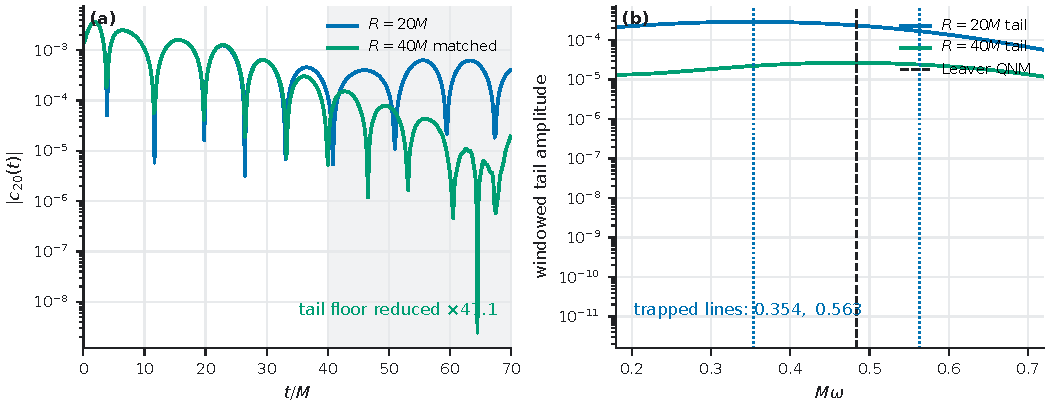
\includegraphics[width=\textwidth]{figures/cavity_domain.pdf}
  \caption{Paired-domain waveform and tail spectrum.  Enlarging the matched
  domain suppresses the finite-domain tail floor, while the small-domain
  spectrum contains two persistent trapped lines.  The marked lines are
  finite-domain cavity modes, not physical QNMs; the Leaver frequency is
  shown only as the physical reference.}
  \label{fig:cavity}
\end{figure*}

Figure~\ref{fig:cavity} shows the paired waveform and tail spectrum.
% numbers.json::domain_R40_lc1match_tail_floor_reduction
% numbers.json::domain_R40_lc1match_R20_peak_over_floor
% numbers.json::domain_R40_lc1match_R40_peak_over_floor
The matched enlargement reduces the tail floor by a factor
$\DomainFloorReductionLcOne$ and raises peak-to-floor from
$\DomainPeakFloorRTwenty$ to $\DomainPeakFloorRForty$.
% numbers.json::cavity_lc1_w1
% numbers.json::cavity_lc1_w2
The small-domain lines are
$M\omega_1=\CavityLcOneWOne\pm\CavityLcOneWOneUnc$ and
$M\omega_2=\CavityLcOneWTwo\pm\CavityLcOneWTwoUnc$.
They are trapped-domain diagnostics, not physical quasinormal frequencies.
% numbers.json::domain_R40_lc1match_delta_re
The matched-domain real-frequency shift,
$\Delta\mathrm{Re}(M\omega)=\DomainDeltaRe\pm\DomainDeltaReUnc$, remains
within the window scatter.

\section{Discussion}
\label{sec:discussion}

The central result is not equality of the two potentials to arbitrary
precision.  It is the persistence of the same logarithmic asymptotic
coefficient at order unity for identical data, in all measured multipoles,
with a separately measured error budget.  Absolute three-dimensional-to-one-
dimensional deviations are larger than the rung-to-rung spread of the paired
discriminator because correlated mesh and estimator errors cancel to first
order in the pair.

% numbers.json::o1_deficit_fraction_explained
% numbers.json::o1_remaining_l2_deficit
The monopole calibration classifies the window bias as a partial explanation:
it accounts for $\OOneDeficitExplained\%$ of the $L^2$ deficit on common
support and leaves $\OOneDeficitResidual$ percentage points.  The residual
is therefore carried as a genuine three-dimensional mesh/extraction
systematic.  We do not use the corrected diagnostic as a replacement result,
and we do not transfer it to $l>0$.

This behavior is complementary to exterior symmetry-restoration studies
\cite{TraykovaBradenPeiris2018,MarsdenEtAl2025}.  Near the horizon, redshift
and accretion can delay or reorganize vacuum dynamics; deeper inside, our
fixed-background calculation shows that the coefficient controlling the
singular profile is instead dominated by the common kinetic evolution.
Modified-gravity scenarios can produce qualitatively different conclusions.
For example, Bars finds Higgs-controlled extensions through the singularity
in a locally conformal framework with antigravity sectors
\cite{Bars2025}.  That contrast does not compete with the present result:
our claim is explicitly restricted to a minimally coupled scalar on a fixed
GR background.

The main limitations are accordingly clear.  Backreaction is absent; the
calculation does not decide the geometry of a self-gravitating singularity.
The radial fit covers a finite interval rather than the mathematical limit.
The $l>0$ truth-window floors prevent a citable profile correction.  The
interior strong phase ends before the late quasi-stationary regime, and the
exterior damping uncertainty remains protocol dominated.  Finally, the
$l$-dependent oscillation cross-check suggested by
Ref.~\cite{ThuestadKhannaPrice2017} would require promoting additional
versioned $l>0$ profile series and is deferred.

\section{Conclusions}
\label{sec:conclusions}

We have extracted the Fournodavlos--Sbierski logarithmic coefficient from
three-dimensional finite-element evolutions inside Schwarzschild and compared
a free scalar with a symmetry-breaking scalar using identical data.
% numbers.json::disc_l0_lc0.028_l2_ratio_frozen
% numbers.json::disc_l1_lc0.040_l2_ratio_frozen
% numbers.json::disc_l2_lc0.028_l2_ratio_frozen
The frozen primary ratios $\DiscLZero$, $\DiscLOne$, and $\DiscLTwo$ show
that the nonlinear vacuum structure does not generate a parametrically
different near-singularity profile in $l=0,1,2$.  A conservative calibration
isolates part of the monopole window bias without promoting a correction
beyond its support.  Independent exterior spectroscopy reproduces the
Schwarzschild QNM within a protocol-dominated uncertainty and exposes both
the unresolved-overtone bias and a finite-domain cavity floor.  Together,
these results support kinetic-domination erasure of vacuum structure in the
test-field Schwarzschild interior while making the Cowling limit and all
resolved systematics explicit.

\bibliography{refs}

\end{document}
